%% A Formalization of Kakutani's Dichotomy for Infinite Product Measures
%% Draft for revision. LIPIcs (ITP/CPP style). Build: tectonic main.tex
\documentclass[a4paper,UKenglish,autoref,thm-restate]{lipics-v2021}

\usepackage{stmaryrd} % \bigsqcap for the Lean iInf glyph
\usepackage{booktabs}

%% ---------------------------------------------------------------------------
%% Lean listings. The Lean source is UTF-8; tectonic's engine passes Unicode
%% characters straight to the T1 text fonts inside verbatim material, so each
%% non-ASCII character in a listing is written as an @-escape to the math
%% glyph instead (mechanically generated from the verbatim Lean source; the
%% rendered output is the source, glyph for glyph).
%% ---------------------------------------------------------------------------
\lstdefinelanguage{lean}{
  morekeywords={theorem,lemma,def,noncomputable,variable,instance,private,
    open,namespace,end,import,fun,Prop,Type,where,deriving},
  sensitive=true,
  morecomment=[l]{--},
  morecomment=[s]{/-}{-/},
  morestring=[b]",
}
\lstset{
  language=lean,
  basicstyle=\small\ttfamily,
  keywordstyle=\bfseries,
  commentstyle=\itshape,
  columns=fullflexible,
  keepspaces=true,
  showstringspaces=false,
  xleftmargin=1em,
  escapechar=@,
}

\newcommand{\ennreal}{\ensuremath{\mathbb{R}_{\ge 0}^{\infty}}}
% \leanid: Lean identifiers in prose; underscores permit a line break, since
% many Mathlib names are longer than a text line can absorb.
\newcommand{\leanid}[1]{{\def\_{\textunderscore\allowbreak}\texttt{#1}}}

\bibliographystyle{plainurl}

\title{A Formalization of Kakutani's Dichotomy for Infinite Product Measures}
\titlerunning{A Formalization of Kakutani's Dichotomy}

%% TODO(author): confirm affiliation line and add ORCID if available.
\author{Daniel Rodriguez}{Independent researcher}{sadasant@gmail.com}{}{}
\authorrunning{D.\ Rodriguez}

\Copyright{Daniel Rodriguez}

\ccsdesc[500]{Theory of computation~Logic and verification}
\ccsdesc[300]{Mathematics of computing~Probability and statistics}

\keywords{Kakutani dichotomy, infinite product measures, Hellinger affinity, measure theory, Lean, Mathlib}

\supplementdetails[subcategory={Source Code}]{Software}{https://github.com/idolum-ai/riemann-venue}

\acknowledgements{This formalization was developed in the \texttt{riemann-venue}
repository by the author in collaboration with Claude Fable 5 (Anthropic), which
co-developed the Lean proofs, computational experiments, and research notes in
interactive sessions under the author's direction and scope decisions
throughout. GPT 5.5 Pro (OpenAI) provided feedback on the accompanying essay and
on the repository's initial outline. All mathematical content is machine-checked
or explicitly labeled otherwise; correctness rests on the Lean kernel and the
reproducibility scripts, not on trust in any author, human or artificial.}

%% TODO(venue): event metadata placeholders; set when the venue is fixed.
\EventEditors{(Editors TBD)}
\EventNoEds{2}
\EventLongTitle{(Venue TBD; prepared in LIPIcs style for an ITP/CPP-type submission)}
\EventShortTitle{TBD 2026}
\EventAcronym{TBD}
\EventYear{2026}
\EventDate{TBD}
\EventLocation{TBD}
\EventLogo{}
\SeriesVolume{0}
\ArticleNo{0}

\begin{document}

\maketitle

\begin{abstract}
Kakutani's dichotomy (1948) states that an infinite product of probability
measures is either absolutely continuous or mutually singular with respect to a
second such product built from pairwise locally absolutely continuous factors,
according to whether the infinite product of the Hellinger affinities of the
factor pairs is positive or zero. We present a formalization of both directions
of the theorem in Lean~4 over Mathlib, stated for families indexed by an
arbitrary type; to the authors' knowledge this is the first formalization of the
theorem in any proof assistant. The development defines the Hellinger affinity
as a total \ennreal-valued function of a pair of measures, proves the singular
direction by a cylinder squeeze and the Borel--Cantelli lemma, and proves the
absolutely continuous direction by a quantitative comparison of the product
measure with a finite-window density measure over the measure-dense algebra of
cylinders. Martingale convergence, the Kolmogorov zero--one law, and
$L^p$-completeness arguments are not used. As an application, a family of
product Poisson measures on an infinite-dimensional torus indexed by the primes
is shown to be mutually singular with product Haar measure exactly for
parameters $\sigma \le 1/2$ and equivalent to it exactly for $\sigma > 1/2$.
The development carries a zero-\texttt{sorry} continuous-integration policy,
and the main theorems depend only on the axioms \texttt{propext},
\texttt{Classical.choice}, and \texttt{Quot.sound}. Upstreaming to Mathlib is
planned as a sequence of six pull requests.
\end{abstract}

\section{Introduction}
\label{sec:intro}

Let $(\Omega_i)_{i \in \iota}$ be measurable spaces carrying two families of
probability measures $\mu_i$ and $\nu_i$ with $\mu_i \ll \nu_i$ for every $i$,
and let $\mu = \bigotimes_i \mu_i$ and $\nu = \bigotimes_i \nu_i$ be the product
measures on $\prod_i \Omega_i$. Kakutani's theorem \cite{kakutani1948} says
that the relationship between $\mu$ and $\nu$ is decided by a single numerical
invariant, the infinite product of the Hellinger affinities
$H(\mu_i, \nu_i) = \int \sqrt{\smash[b]{\tfrac{d\mu_i}{d\nu_i}}}\, d\nu_i$: if
$\prod_i H(\mu_i,\nu_i) > 0$ then $\mu \ll \nu$, and if the product is $0$ then
$\mu$ and $\nu$ are mutually singular. When each pair is mutually absolutely
continuous, the conclusion sharpens to a dichotomy between equivalence and
mutual singularity, with no intermediate regime.

The theorem is a standard instrument of measure-theoretic probability. It is
the ancestor of the Feldman--H\'ajek dichotomy for Gaussian measures
\cite{feldman1958,hajek1958}, it governs when two stochastic models with
independent coordinates can be distinguished with certainty from a single
sample, and its criterion is effective: since $0 \le H(\mu_i,\nu_i) \le 1$, the
product is positive precisely when the deficits $1 - H(\mu_i,\nu_i)$ are
summable, so verifying either branch of the dichotomy reduces to a convergence
estimate.

To our knowledge the theorem had no formalization in any proof assistant before
this work; \autoref{sec:related} and \autoref{sec:artifact} record the basis
for this claim and the protocol for re-verifying it prior to publication. One
structural reason is that the statement needs infinite products of probability
measures over arbitrary index sets as first-class objects, and Lean's Mathlib
\cite{mathlib2020,demoura2021} acquired these only recently
(\leanid{Measure.infinitePi}, built through the Ionescu--Tulcea theorem
\cite{ionescutulcea1949}). A second reason is that the textbook proofs
\cite{williams1991} run through martingale convergence and $L^2$ limit
arguments, which are formalizable but drag in machinery whose bookkeeping
dominates the mathematics. The routes chosen here avoid that machinery
entirely.

The contributions:
\begin{itemize}
\item Machine-checked statements and proofs of both directions of Kakutani's
  dichotomy in Lean~4 over Mathlib, for factor families indexed by an
  \emph{arbitrary} type. This is stronger than the classical countable
  statement, and it fell out of the proof routes rather than being a goal.
\item A reusable definition of the Hellinger affinity as a total,
  \ennreal-valued, symmetric function of a pair of measures, with its basic
  API, including $H(\mu,\nu) = 0 \leftrightarrow \mu \perp \nu$
  (\autoref{sec:affinity}).
\item Supporting lemmas absent from Mathlib at the pinned revision: finite
  tensorization of densities (\leanid{Measure.pi\_withDensity}), a product
  Fubini theorem for the lower Lebesgue integral, positivity and summability
  bridges for infinite products in \ennreal, and window-factorization lemmas
  over \leanid{Measure.infinitePi} (\autoref{sec:formalization}).
\item Proof routes suited to formalization: the singular direction by a
  cylinder squeeze and Borel--Cantelli, the absolutely continuous direction by
  a quantitative cylinder comparison. Neither uses martingales, the zero--one
  law, or $L^p$ completeness (\autoref{sec:engineering}).
\item An application: the family of product Poisson measures over the primes at
  ratios $p^{-\sigma}$ changes type against product Haar measure exactly at
  $\sigma = 1/2$ (\autoref{sec:application}).
\item A public artifact with zero-\texttt{sorry} CI, axiom audits, and a
  staged plan for upstreaming the general-purpose layer to Mathlib
  (\autoref{sec:artifact}).
\end{itemize}

The formalization was built as an instrument for a research program on the
spectral geometry of the greatest-common-divisor kernel \cite{riemannvenue};
\autoref{sec:application} states the one theorem of that program that this
paper reports.

\section{Mathematical background}
\label{sec:background}

\subsection{The Hellinger affinity}

For probability measures $\mu, \nu$ on a measurable space $\Omega$ and any
$\sigma$-finite measure $\lambda$ dominating both, the \emph{Hellinger
affinity} (also the Bhattacharyya coefficient
\cite{hellinger1909,bhattacharyya1943}) is
\[
  H(\mu, \nu) \;=\; \int_\Omega \sqrt{\frac{d\mu}{d\lambda}\cdot
  \frac{d\nu}{d\lambda}} \; d\lambda ,
\]
independent of the choice of $\lambda$. It is symmetric, and by
Cauchy--Schwarz $0 \le H(\mu,\nu) \le 1$, with $H(\mu,\mu) = 1$. The two
endpoints carry the geometry: $H(\mu,\nu) = 1$ iff $\mu = \nu$, and
$H(\mu,\nu) = 0$ iff $\mu \perp \nu$. The affinity tensorizes over finite
products, $H(\mu_1 \otimes \mu_2, \nu_1 \otimes \nu_2) = H(\mu_1,\nu_1) \cdot
H(\mu_2,\nu_2)$, which is what makes it the right invariant for product
measures.

\subsection{The dichotomy}

\begin{theorem}[Kakutani \cite{kakutani1948}]
\label{thm:kakutani}
For each $i$ in a countable index set let $\mu_i, \nu_i$ be probability
measures on $\Omega_i$ with $\mu_i \ll \nu_i$, and set
$\mu = \bigotimes_i \mu_i$, $\nu = \bigotimes_i \nu_i$.
\begin{enumerate}
\item If $\prod_i H(\mu_i, \nu_i) > 0$, then $\mu \ll \nu$.
\item If $\prod_i H(\mu_i, \nu_i) = 0$, then $\mu \perp \nu$.
\end{enumerate}
If moreover $\nu_i \ll \mu_i$ for every $i$, the first case gives equivalence
of $\mu$ and $\nu$.
\end{theorem}

Since every factor lies in $[0,1]$, the partial products are antitone and the
infinite product converges to a limit in $[0,1]$; positivity of the limit is
equivalent to summability of the deficits:
\[
  \prod_i H(\mu_i,\nu_i) > 0
  \quad\Longleftrightarrow\quad
  \sum_i \bigl(1 - H(\mu_i,\nu_i)\bigr) < \infty
  \;\text{ and }\; H(\mu_i,\nu_i) > 0 \text{ for all } i .
\]

The classical proof \cite{kakutani1948,williams1991} considers the likelihood
ratios $Z_n = \prod_{i \le n} \frac{d\mu_i}{d\nu_i}$, a nonnegative
$\nu$-martingale. In the convergent case the square roots $\sqrt{Z_n}$ form a
Cauchy sequence in $L^2(\nu)$, the limit identifies $\frac{d\mu}{d\nu}$, and
absolute continuity follows; in the divergent case $Z_n \to 0$ almost
everywhere under $\nu$ while $\mu$ concentrates where $Z_n$ survives, and a
zero--one argument upgrades this to mutual singularity. The formalized proofs
reach the same conclusions along different routes
(\autoref{sec:engineering}).

\section{The formalization}
\label{sec:formalization}

The development comprises six Lean files plus two application files under
\texttt{RiemannVenue/}\allowbreak\texttt{Kakutani/} in the artifact \cite{riemannvenue}, built
against a pinned Mathlib revision (\autoref{sec:artifact}). Everything in this
section and the next lives in the \leanid{MeasureTheory} namespace, most of it
under \leanid{Measure}; the application (\autoref{sec:application}) lives in
the repository's own namespace. \autoref{fig:ladder} shows the
milestone ladder; each box was designed, then implemented as one complete file
with no placeholders.

\begin{figure}[t]
  \centering
  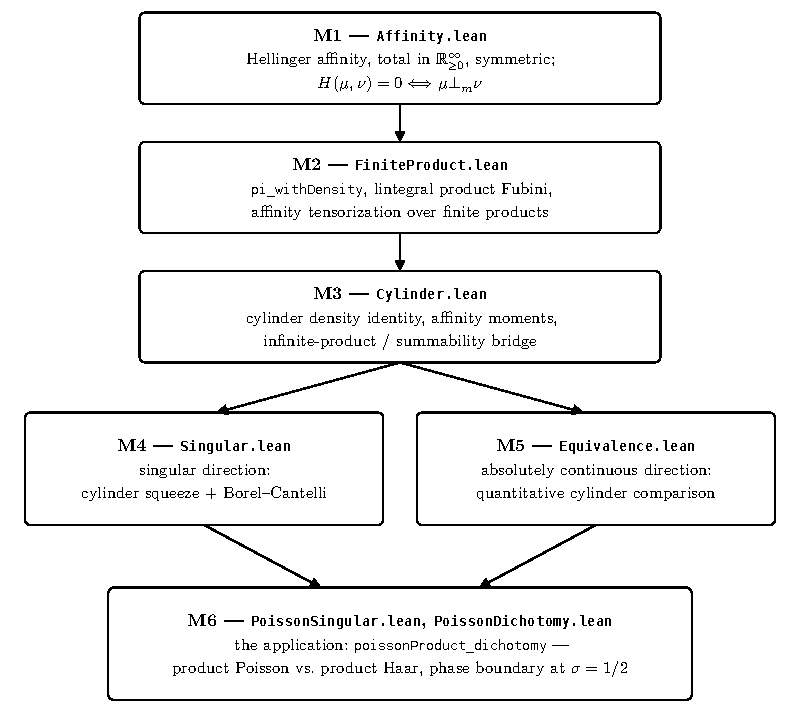
\includegraphics[width=0.78\linewidth]{figures/ladder.pdf}
  \caption{The milestone ladder. M1--M3 are infrastructure, M4 and M5 are the
  two directions of the dichotomy (independent of one another), M6 is the
  application. Arrows are import dependencies.}
  \label{fig:ladder}
\end{figure}

\subsection{Infinite product measures in Mathlib}

Mathlib's \leanid{Measure.infinitePi} takes an arbitrary index type $\iota$
and a family $\mu : (i : \iota) \to \leanid{Measure}\,(X\,i)$ of probability
measures, and produces the product probability measure on $\Pi_i\, X\,i$. The
$\mathbb{N}$-indexed core is the projective limit supplied by the
Ionescu--Tulcea theorem \cite{ionescutulcea1949}; the general case is a
Carath\'eodory extension of the induced content on measurable cylinders. The
API this development consumes is the cylinder evaluation
(\leanid{infinitePi\_cylinder}), the finite-marginal identification
(\leanid{infinitePi\_map\_restrict}), and the restriction rule for lower
Lebesgue integrals of finite-window functions
(\leanid{lintegral\_restrict\_infinitePi}). The recency of this layer is the
main reason a 1948 theorem was still open to formalization.

\subsection{The Hellinger affinity as formalized}
\label{sec:affinity}

\begin{lstlisting}
/-- The Hellinger affinity (Bhattacharyya coefficient) of two measures:
`@$\int$@ @$\surd$@(d@$\mu$@/d@$\sigma$@ @$\cdot$@ d@$\nu$@/d@$\sigma$@) d@$\sigma$@` computed against the canonical dominating measure
`@$\sigma$@ = @$\mu$@ + @$\nu$@`. Total and symmetric; no absolute-continuity hypothesis. -/
noncomputable def hellingerAffinity (@$\mu$@ @$\nu$@ : Measure @$\Omega$@) : @$\mathbb{R}$@@$\ge$@0@$\infty$@ :=
  @$\int$@@${}^{-}$@ x, (@$\mu$@.rnDeriv (@$\mu$@ + @$\nu$@) x * @$\nu$@.rnDeriv (@$\mu$@ + @$\nu$@) x) ^ (1 / 2 : @$\mathbb{R}$@) @$\partial$@(@$\mu$@ + @$\nu$@)
\end{lstlisting}

Three design decisions are packed into this definition. First, the dominating
measure is fixed to $\mu + \nu$, so the affinity is total: it needs no
absolute-continuity or integrability hypotheses, and an invariance lemma
(\leanid{hellingerAffinity\_eq\_lintegral\_rnDeriv\_mul\_rnDeriv}) recovers the
value against any dominating $\sigma$-finite measure. Second, the value type
is \ennreal{} and the integral is the lower Lebesgue integral, so no side
conditions about integrability arise anywhere in the development; Mathlib's
Kullback--Leibler divergence \leanid{klDiv} made the same choice. Third,
totality is what makes the singular direction of the dichotomy free of case
splits: the characterization
\begin{lstlisting}
theorem hellingerAffinity_eq_zero_iff [IsFiniteMeasure @$\mu$@] [IsFiniteMeasure @$\nu$@] :
    hellingerAffinity @$\mu$@ @$\nu$@ = 0 @$\leftrightarrow$@ @$\mu$@ @$\perp$@@${}_{m}$@ @$\nu$@
\end{lstlisting}
holds with no hypotheses beyond finiteness, so degenerate factor pairs need no
separate treatment. The remaining API proves symmetry, $H(\mu,\mu) = 1$,
$H(\mu,\nu) \le 1$ (H\"older with exponents $2, 2$), the computation rules
under $\mu \ll \nu$ and for \leanid{withDensity} reweightings, and
tensorization over finite products
(\leanid{hellingerAffinity\_pi}).

\subsection{The hypothesis carrier: infima of partial products}
\label{sec:carrier}

The dichotomy's hypothesis is the value of an infinite product. Mathlib's
\leanid{tprod} is unsuitable as a carrier for it: like \leanid{tsum}, it
returns the junk value $1$ for non-multipliable families, and ``the infinite
product is $0$'' is exactly the case where multipliability fails. Since every
factor is $\le 1$, the finite partial products form an antitone net, and its
infimum is the honest value of the infinite product. The formalized
statements therefore quantify over finite subsets:
\[
  \bigsqcap_{s : \leanid{Finset}\ \iota}\ \prod_{i \in s}
  H(\mu_i, \nu_i)
  \;=\; 0
  \qquad\text{versus}\qquad
  0 \;<\; \bigsqcap_{s}\ \prod_{i \in s} H(\mu_i, \nu_i).
\]
A bridge lemma converts between this form and the summability criterion:
\begin{lstlisting}
theorem iInf_finsetProd_pos_iff_summable_one_sub {h : @$\kappa$@ @$\to$@ @$\mathbb{R}$@@$\ge$@0@$\infty$@}
    (h1 : @$\forall$@ i, h i @$\le$@ 1) :
    (0 < @$\bigsqcap$@ s : Finset @$\kappa$@, @$\prod$@ i @$\in$@ s, h i)
      @$\leftrightarrow$@ (@$\forall$@ i, h i @$\ne$@ 0) @$\wedge$@ Summable fun i => 1 - (h i).toReal
\end{lstlisting}
Its proof rests on two elementary inequalities, formalized over the reals: the
Weierstrass bound $1 - \prod_{i \in s} h_i \le \sum_{i \in s} (1 - h_i)$ and
the exponential bound $\prod_{i \in s} h_i \le \exp\bigl(-\sum_{i \in s} (1 -
h_i)\bigr)$.

\subsection{The main statements}
\label{sec:statements}

The following are quoted verbatim from the artifact. The ambient context is
\begin{lstlisting}
variable {@$\iota$@ : Type*} {X : @$\iota$@ @$\to$@ Type*} {mX : @$\forall$@ i, MeasurableSpace (X i)}
  (@$\mu$@ @$\nu$@ : (i : @$\iota$@) @$\to$@ Measure (X i))
  [@$\forall$@ i, IsProbabilityMeasure (@$\mu$@ i)] [@$\forall$@ i, IsProbabilityMeasure (@$\nu$@ i)]
\end{lstlisting}
with no constraint on $\iota$. The singular direction
(\texttt{Singular.lean}):
\begin{lstlisting}
theorem infinitePi_mutuallySingular (hac : @$\forall$@ i, @$\mu$@ i @$\ll$@ @$\nu$@ i)
    (h : @$\bigsqcap$@ s : Finset @$\iota$@, @$\prod$@ i @$\in$@ s, hellingerAffinity (@$\mu$@ i) (@$\nu$@ i) = 0) :
    Measure.infinitePi @$\mu$@ @$\perp$@@${}_{m}$@ Measure.infinitePi @$\nu$@
\end{lstlisting}
The absolutely continuous direction, in its summability and infimum forms, and
the two-sided corollary under mutual local absolute continuity
(\texttt{Equivalence.lean}):
\begin{lstlisting}
theorem infinitePi_absolutelyContinuous_of_summable (hac : @$\forall$@ i, @$\mu$@ i @$\ll$@ @$\nu$@ i)
    (hsum : Summable fun i => 1 - (hellingerAffinity (@$\mu$@ i) (@$\nu$@ i)).toReal) :
    Measure.infinitePi @$\mu$@ @$\ll$@ Measure.infinitePi @$\nu$@

theorem infinitePi_absolutelyContinuous (hac : @$\forall$@ i, @$\mu$@ i @$\ll$@ @$\nu$@ i)
    (h : 0 < @$\bigsqcap$@ s : Finset @$\iota$@, @$\prod$@ i @$\in$@ s, hellingerAffinity (@$\mu$@ i) (@$\nu$@ i)) :
    Measure.infinitePi @$\mu$@ @$\ll$@ Measure.infinitePi @$\nu$@

theorem infinitePi_absolutelyContinuous_and_symm
    (hac : @$\forall$@ i, @$\mu$@ i @$\ll$@ @$\nu$@ i) (hac' : @$\forall$@ i, @$\nu$@ i @$\ll$@ @$\mu$@ i)
    (h : 0 < @$\bigsqcap$@ s : Finset @$\iota$@, @$\prod$@ i @$\in$@ s, hellingerAffinity (@$\mu$@ i) (@$\nu$@ i)) :
    Measure.infinitePi @$\mu$@ @$\ll$@ Measure.infinitePi @$\nu$@ @$\wedge$@
      Measure.infinitePi @$\nu$@ @$\ll$@ Measure.infinitePi @$\mu$@
\end{lstlisting}

Two remarks on the hypotheses, in the interest of precision. The index type is
arbitrary in both directions; \autoref{sec:engineering} explains why
countability is never needed. And the singular direction carries the local
absolute-continuity hypothesis \leanid{hac} even though the affinity was
defined so as not to need it: the hypothesis enters only because the finite
window densities are built from \leanid{rnDeriv} against $\nu_i$. The singular
parts of the $\mu_i$ can only help singularity, so the hypothesis is
removable; the generalization is recorded in the file's docstring and deferred
to the Mathlib port (\autoref{sec:artifact}). For the same reason, the
packaged disjunction (``absolutely continuous or mutually singular'') is not a
separate declaration in the artifact; under \leanid{hac} it is a two-line
order split on the infimum, and it is scheduled to be added, in that packaged
form, during the port. A degenerate-case lemma is included: if any single
factor pair is mutually singular, the products are
(\leanid{infinitePi\_mutuallySingular\_of\_mutuallySingular}), with no
absolute-continuity hypothesis at all.

\section{Proof engineering}
\label{sec:engineering}

\begin{figure}[t]
  \centering
  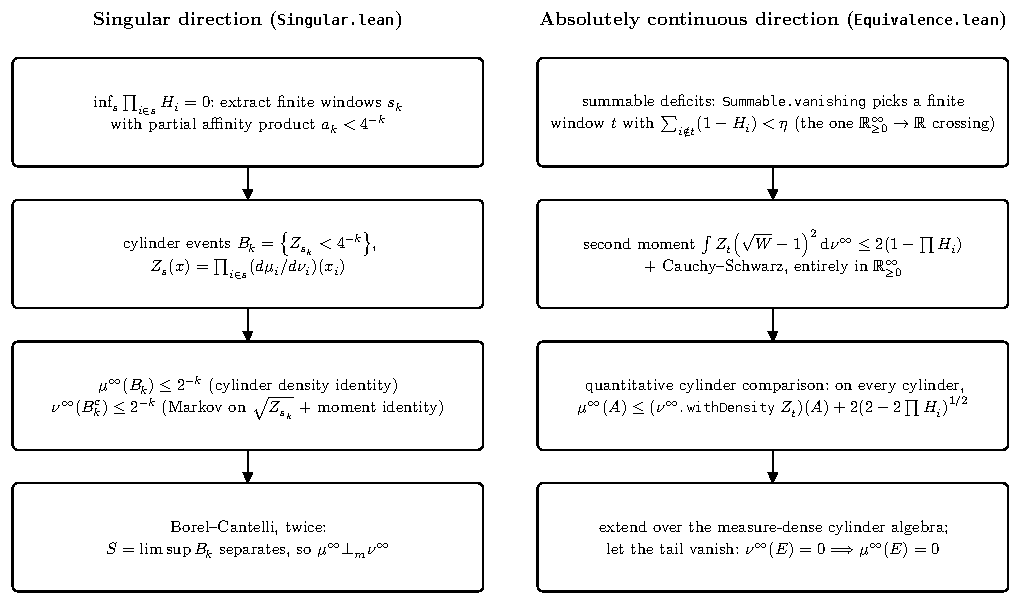
\includegraphics[width=\linewidth]{figures/routes.pdf}
  \caption{The two proof routes. Here $H_i = \leanid{hellingerAffinity}\,
  (\mu\,i)\,(\nu\,i)$, $Z_s$ is the finite-window likelihood ratio, $W$ the
  ratio over a window disjoint from $t$, and $\mu^\infty, \nu^\infty$ the
  infinite product measures.}
  \label{fig:routes}
\end{figure}

Both routes are summarized in \autoref{fig:routes}. The design constraint
common to both: keep every estimate in \ennreal{} as long as possible, because
each crossing between \ennreal{} and $\mathbb{R}$ costs finiteness and
nonnegativity side conditions, and those crossings are where formalized
analysis stalls.

\subsection{The singular direction: cylinder squeeze and Borel--Cantelli}
\label{sec:singular-route}

Suppose the infimum of partial affinity products is $0$. For each $k$ extract
a finite window $s_k$ with $\prod_{i \in s_k} H_i < 4^{-k}$, and consider the
cylinder event $B_k = \{x \mid Z_{s_k}(x) < 4^{-k}\}$ where
$Z_s(x) = \prod_{i \in s}\frac{d\mu_i}{d\nu_i}(x_i)$. Two one-line estimates
squeeze this event from both sides:
\begin{itemize}
\item $\mu^\infty(B_k) \le 4^{-k} \le 2^{-k}$, because the cylinder density
  identity (\leanid{infinitePi\_cylinder\_eq\_setLIntegral\_rnDeriv},
  file \texttt{Cylinder.lean}) evaluates $\mu^\infty$ on a cylinder as the
  $\nu^\infty$-integral of $Z_{s_k}$ over it, and the integrand is below
  $4^{-k}$ there;
\item $\nu^\infty(B_k^{\,c}) \le 2^{-k}$, by Markov's inequality applied to
  $\sqrt{Z_{s_k}}$ together with the moment identity
  $\int \sqrt{Z_s}\, d\nu^\infty = \prod_{i \in s} H_i$
  (\leanid{lintegral\_prod\_rnDeriv\_rpow\_infinitePi}).
\end{itemize}
Both bounds are geometrically summable, so the Borel--Cantelli lemma applies
twice: $S = \limsup_k B_k$ is $\mu^\infty$-null, and its complement, contained
in $\limsup_k B_k^{\,c}$, is $\nu^\infty$-null. The set $S$ witnesses mutual
singularity directly.

This route uses no martingale convergence and no zero--one law, although both
exist in Mathlib and were mapped as fallbacks during design. The payoff is
concrete: the entire proof is elementary integration against cylinders, and it
is the reason the statement holds for arbitrary $\iota$, since only a
\emph{sequence} of finite windows is ever extracted from the vanishing
infimum.

\subsection{The absolutely continuous direction: quantitative comparison}
\label{sec:ac-route}

The classical route builds $\lim_n \sqrt{Z_n}$ in $L^2(\nu^\infty)$ and
identifies its square as the density of $\mu^\infty$. Formalizing it means
moving between \ennreal-valued densities and real-valued $L^2$ functions
repeatedly. The implemented route instead compares measures directly. Its
core is a quantitative estimate (\texttt{Equivalence.lean}):
\begin{lstlisting}[basicstyle=\footnotesize\ttfamily]
theorem infinitePi_cylinder_le_withDensity_add [DecidableEq @$\iota$@]
    (hac : @$\forall$@ i, @$\mu$@ i @$\ll$@ @$\nu$@ i) {t u : Finset @$\iota$@} (htu : t @$\subseteq$@ u)
    {S : Set (@$\Pi$@ i : u, X i)} (hS : MeasurableSet S) :
    Measure.infinitePi @$\mu$@ (cylinder u S)
      @$\le$@ (Measure.infinitePi @$\nu$@).withDensity
            (fun x => @$\prod$@ i @$\in$@ t, (@$\mu$@ i).rnDeriv (@$\nu$@ i) (x i)) (cylinder u S)
          + 2 * (2 - 2 * @$\prod$@ i @$\in$@ u \ t, hellingerAffinity (@$\mu$@ i) (@$\nu$@ i)) ^ (1 / 2 : @$\mathbb{R}$@)
\end{lstlisting}
On any cylinder, $\mu^\infty$ exceeds the finite-window density measure
$\nu^\infty.\leanid{withDensity}\,Z_t$ by at most an error controlled by the
affinity product over the coordinates beyond $t$. The proof is the classical
second-moment computation in disguise: with $W$ the likelihood ratio over
$u \setminus t$ and $c = \sqrt{W}$, the factorization of window moments over
disjoint windows (\leanid{lintegral\_prod\_mul\_prod\_infinitePi}) gives
$\int Z_t (c-1)^2 \, d\nu^\infty \le 2 - 2\prod_{i \in u \setminus t} H_i$,
and two applications of Cauchy--Schwarz for the lower Lebesgue integral
convert this into the additive bound. Every step is in \ennreal; subtraction
is truncated, and three small helper lemmas manage the truncation
arithmetic.

The extension from cylinders to all measurable sets is a symmetric-difference
approximation: measurable cylinders form a set algebra generating the product
$\sigma$-algebra, and Mathlib's \leanid{MeasureDense} machinery shows every
measurable set is approximated in measure by cylinders. A short lemma
(\leanid{measure\_le\_add\_of\_le\_add\_on\_setAlgebra}) transports the bound
``$m_1 \le m_2 + \beta$ on a generating algebra'' to all measurable sets.
Given $\nu^\infty(E) = 0$ and $\varepsilon > 0$, summability of the deficits
supplies, through \leanid{Summable.vanishing}, a finite window $t$ whose tail
contributes less than $\varepsilon$; the density measure vanishes on $E$
because $\nu^\infty$ does, and $\mu^\infty(E) \le \varepsilon$ follows. The
only crossing from \ennreal{} to $\mathbb{R}$ in the whole direction is the
Weierstrass bridge inside the tail estimate.

Countability of $\iota$ is again never used: a summable deficit family is
supported on countably many indices without any need to say so, because the
argument only ever selects finite windows. The design documents anticipated a
reduction of countable $\iota$ to $\mathbb{N}$ by re-indexing; the implemented
route made it unnecessary, and the stated theorems are stronger than the
designed ones.

\subsection{Method: scout first, then implement}
\label{sec:method}

The development was written design-first. Before any Lean file was created, a
design document fixed the definitions, the statement shapes, the milestone
ladder of \autoref{fig:ladder}, and, for every milestone, the exact Mathlib
lemmas to be consumed, each verified by \texttt{grep} against the pinned
Mathlib revision and recorded with file and line. The document also carried a
risk register with ordered fallbacks. Implementation then proceeded one
milestone at a time, each landing as a complete file with no
\texttt{sorry}; the waves compiled green on the first or near-first attempt.

The register is worth reporting because two of its entries fired. The risk
item for the absolutely continuous direction predicted that
\ennreal/$\mathbb{R}$ bookkeeping would dominate an $L^2$ route and prescribed
keeping all cylinder identities in \ennreal{} with a single crossing;
following that prescription to its end produced the comparison route of
\autoref{sec:ac-route}, and the $L^2$ machinery was never needed. The risk
item for the application predicted friction in a quotient-circle
(\leanid{AddCircle}) model and named an interval model as fallback; the
fallback was taken directly (\autoref{sec:application}). The residue of the
one pinned-toolchain workaround that remains
(a \leanid{set\_option} guarding one Fubini proof) is flagged in the
upstreaming plan.

\section{Application: a phase boundary at the critical exponent}
\label{sec:application}

The repository \cite{riemannvenue} studies the kernel
$K(m,n) = \gcd(m,n)/\sqrt{mn}$ and its spectral representations. One of them
realizes $K$ through Fourier coefficients of a product Poisson measure on an
infinite-dimensional torus indexed by the primes, with per-prime radii
$a_p = p^{-\sigma}$. The local model at each prime, kept on $\mathbb{R}$
rather than on a quotient circle, is:
\begin{lstlisting}
noncomputable def haarIoc : Measure @$\mathbb{R}$@ :=
  (ENNReal.ofReal (2 * Real.pi))@${}^{-}$@@${}^{1}$@ @$\bullet$@ volume.restrict (Set.Ioc (-Real.pi) Real.pi)

noncomputable def poissonMeasure (a : @$\mathbb{R}$@) : Measure @$\mathbb{R}$@ :=
  haarIoc.withDensity fun @$\theta$@ => ENNReal.ofReal (poissonKernel a @$\theta$@)
\end{lstlisting}
where \leanid{poissonKernel}~$a$~$\theta = (1-a^2)/\lvert 1 - a
e^{i\theta}\rvert^2$ is the classical Poisson kernel, a strictly positive
probability density for $0 < a < 1$. A computation
(\leanid{hellingerAffinity\_poissonMeasure}) identifies the abstract affinity
of the pair with the repository's analytic benchmark value
$\operatorname{hellinger}(a) = (2\pi)^{-1} \int_{-\pi}^{\pi}
\sqrt{P_a(\theta)}\, d\theta$, and an analytic bridge already in the
repository (\leanid{summable\_hellinger\_deficit\_iff}) shows the deficits
$1 - \operatorname{hellinger}(p^{-\sigma})$ are summable over the primes iff
$\sigma > 1/2$, with divergence at the endpoint. The mechanism is the
classical one: the deficit at small $a$ is comparable to $a^2$, so the series
behaves like $\sum_p p^{-2\sigma}$, which converges exactly for
$\sigma > 1/2$ and diverges at $\sigma = 1/2$ like $\sum_p 1/p$.

Feeding this into the two directions of the dichotomy yields the phase
boundary as a single statement (\texttt{PoissonDichotomy.lean}):
\begin{lstlisting}
theorem poissonProduct_dichotomy {@$\sigma$@ : @$\mathbb{R}$@} (h@$\sigma$@@${}_{0}$@ : 0 < @$\sigma$@) :
    (Measure.infinitePi (fun p : Nat.Primes => poissonMeasure ((p : @$\mathbb{R}$@) ^ (-@$\sigma$@)))
        @$\perp$@@${}_{m}$@ Measure.infinitePi (fun _ : Nat.Primes => haarIoc) @$\leftrightarrow$@ @$\sigma$@ @$\le$@ 1 / 2) @$\wedge$@
      (Measure.infinitePi (fun p : Nat.Primes => poissonMeasure ((p : @$\mathbb{R}$@) ^ (-@$\sigma$@)))
        @$\ll$@ Measure.infinitePi (fun _ : Nat.Primes => haarIoc) @$\leftrightarrow$@ 1 / 2 < @$\sigma$@)
\end{lstlisting}
For $\sigma > 1/2$ the two products are in fact equivalent
(\leanid{poissonProduct\_equivalent}); the backward implications are
exclusivity, since a nonzero measure cannot be both absolutely continuous and
mutually singular with respect to the same measure. The type change lands
exactly at the critical exponent, with the endpoint $\sigma = 1/2$ on the
singular side. Within the wider program this theorem is the machine-checked
form of a claim the accompanying essay makes about the log-scale boundary
behavior of the divisibility geometry; the program's other results and its
open problems are catalogued in the repository's status ledger
\cite{riemannvenue} and are out of scope here.

\section{Related work}
\label{sec:related}

Measure and probability theory have mature formalized foundations in several
systems. In Isabelle/HOL, measure theory and the core of probability were
developed by H\"olzl and Heller \cite{hoelzl2011}, and infinite products of
probability measures, via projective limits in the Ionescu--Tulcea style, are
part of H\"olzl's subsequent development \cite{hoelzl2013}; the infrastructure
for stating Kakutani's theorem has therefore existed in Isabelle for some
time. In Coq, MathComp-Analysis provides measure construction and the
Lebesgue integral \cite{affeldtcohen2023}. In Lean, Mathlib
\cite{mathlib2020} contains the Radon--Nikodym theorem, the Lebesgue
decomposition, martingale convergence, and, recently, the infinite product
measures this work builds on. We searched the Isabelle Archive of Formal
Proofs, the Coq ecosystem, and the Lean/Mathlib libraries for a formalization
of Kakutani's theorem and found none; the claim of first formalization is
made to the authors' knowledge, and \autoref{sec:artifact} commits to
re-verifying it immediately before publication.

On the divergence side, Mathlib contains the Kullback--Leibler divergence,
\ennreal-valued and standalone. A broader $f$-divergence framework by Degenne
and Luccioli \cite{testinglowerbounds} exists as an external Lean development
and has begun to be upstreamed; the Hellinger affinity defined here is the
$f$-integral at $f = \sqrt{\cdot\,}$, and a bridging lemma is planned for
whenever the general framework lands (\autoref{sec:artifact}). The
formalization of the Feldman--H\'ajek dichotomy for Gaussian measures
\cite{feldman1958,hajek1958}, for which the present theorem is a natural
stepping stone, remains open in all systems as far as we know.

\section{Artifact and upstreaming}
\label{sec:artifact}

\paragraph*{Artifact.} The development is part of the public repository
\texttt{riemann-venue} \cite{riemannvenue}, Apache-2.0, frozen for this
article at commit \texttt{[COMMIT]}.
%% TODO(author): replace [COMMIT] here and in kakutani.bib at freeze time.
The Kakutani layer is:

\begin{center}
\small
\begin{tabular}{@{}llr@{}}
\toprule
File (\texttt{RiemannVenue/Kakutani/}) & Contents & Lines \\
\midrule
\texttt{Affinity.lean} & Hellinger affinity and API (M1) & 197 \\
\texttt{FiniteProduct.lean} & \leanid{pi\_withDensity}, lintegral Fubini, tensorization (M2) & 143 \\
\texttt{Cylinder.lean} & bridges, cylinder density and moment identities (M3) & 274 \\
\texttt{Singular.lean} & singular direction (M4) & 208 \\
\texttt{Equivalence.lean} & absolutely continuous direction (M5) & 484 \\
\texttt{PoissonSingular.lean} & local Poisson model, singular half of M6 & 218 \\
\texttt{PoissonDichotomy.lean} & equivalence half and the packaged boundary (M6) & 175 \\
\texttt{SpectralMeasure.lean} & Bochner window factorization; spectral application & 248 \\
\bottomrule
\end{tabular}
\end{center}

The toolchain is Lean 4 (\texttt{leanprover/lean4:v4.32.0-rc1}) with Mathlib
pinned at revision \texttt{e2361c1}. Continuous integration builds the full
repository and enforces a zero-\texttt{sorry} policy by a textual guard in
addition to the build. Axiom audits via \leanid{\#print axioms} on the main
declarations (\leanid{infinitePi\_mutuallySingular},
\leanid{infinitePi\_absolutelyContinuous\_of\_summable},
\leanid{poissonProduct\_dichotomy}) report exactly \leanid{propext},
\leanid{Classical.choice}, and \leanid{Quot.sound}. To build:
\begin{lstlisting}[language={}]
lake exe cache get && lake build
\end{lstlisting}

\paragraph*{Upstreaming.} The general-purpose layer (everything except the
Poisson application) is scheduled for Mathlib as six pull requests, about 31
public declarations in total: (1) the Hellinger affinity file; (2)
\leanid{pi\_withDensity} and the lintegral product Fubini; (3) the
infinite-product/summability bridges; (4) the singular direction, with the
\leanid{hac} hypothesis dropped as discussed in \autoref{sec:statements}; (5)
the absolutely continuous direction together with the packaged dichotomy and
the equivalence restated as a biconditional; (6) the Bochner window
factorization over \leanid{infinitePi}, which is independent of the rest.
PRs 1--3 and 6 have no interdependencies; 4 needs 1--3; 5 needs 4. The plan,
including naming deltas, the module-system port, and known drift risks
between the pin and current Mathlib, is a document in the repository
(\texttt{notes/}\allowbreak\texttt{mathlib-pr-plan.md}).

\paragraph*{Verification of the novelty claim.} The claim that no prior
formalization exists will be re-checked against the Isabelle AFP, the Coq
opam ecosystem, and the Lean/Mathlib and Zulip archives immediately before
this article is published in any form, and the hedge ``to the authors'
knowledge'' will be retained regardless of the outcome.

\section{Conclusion}
\label{sec:conclusion}

Kakutani's dichotomy is now a machine-checked theorem, in a form slightly
stronger than the classical one, with proof routes chosen so that the
formalization consists of elementary integration against cylinders rather
than martingale limit theory. The exercise supports a working hypothesis
about formalizing graduate-level measure theory: the cost concentrates at
value-type crossings, and route selection that minimizes those crossings can
matter more than the availability of heavy machinery. Next steps are the
removal of the residual absolute-continuity hypothesis on the singular
direction, the Mathlib pull-request sequence, and, once a general
$f$-divergence framework is in Mathlib, the bridging lemma tying the affinity
to it. The Feldman--H\'ajek dichotomy is the natural continuation.

\bibliography{kakutani}

\end{document}
